\section{Exercise 3: Random asymmetry}

\begin{itshape}
\small
To investigate the robustness of pattern retrieval against asymmetry in the weight matrix, consider now networks where for each pairs of nodes $\l(i, j\r)$, the directed connection from node $i$ to node $j$ is cut with probability $p_{cut}$. This will introduce asymmetry in the Hebbian weight matrix Eq. 1.

Set $c=0.1$ and $N = 200$. As in Ex. 2 calculate and plot the mean $\alpha_{N,max}$ for varying $p_{cut}$ with error bars (at least 10 repetitions). At which $p_{cut}$ does the maximal load drop below $50\%$ of the value estimated in Ex. 2? State the confidence interval.

Note: Bare in mind that the convergence assertion of Question 1.1 does not necessarily hold for $p_{cut} > 0$.
\end{itshape}

\paragraph*{}

\begin{wrapfigure}{r}{0.5\textwidth}
  \vspace{-20pt}
  \begin{center}
%    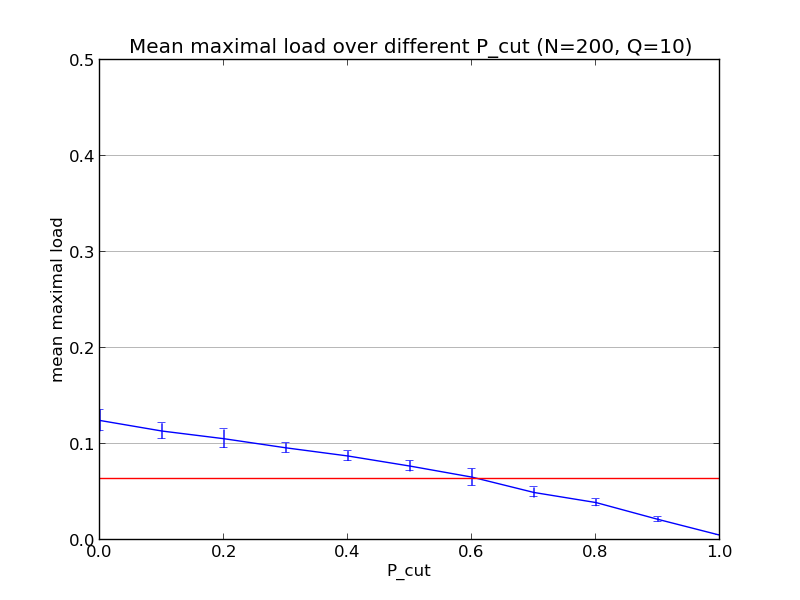
\includegraphics[width=0.6\textwidth]{dat/ex3-mean_max_load-N200-Q10-C95}
  \end{center}
  \vspace{-20pt}
  \caption{Exercise 3: Maximal load $\alpha_{N,max}$ averaged over 10 repetitions for varying $p_{cut}$ }
  \label{fig:exercise3}
  \vspace{-10pt}
\end{wrapfigure}


